\pagenumbering{gobble}
\begin{figure}
  \centering
  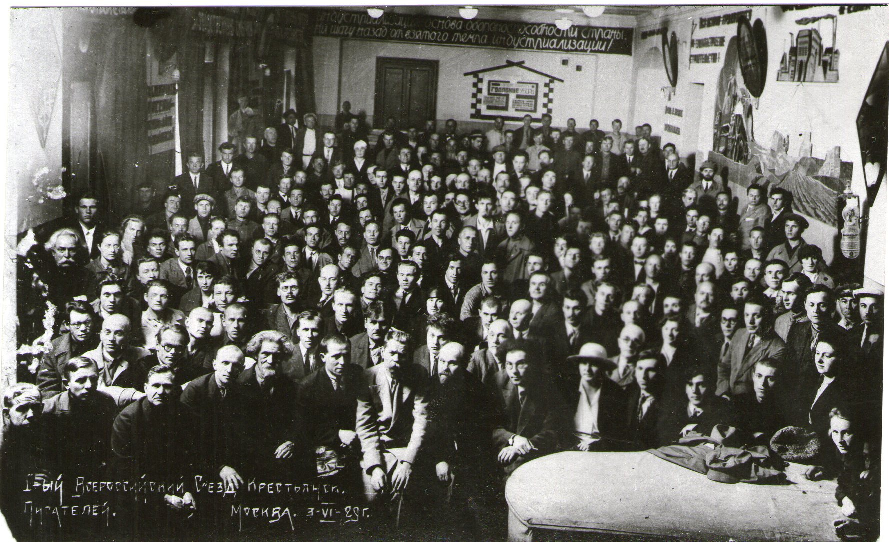
\includegraphics[width=0.9\textwidth]{syezd.pdf}
  \caption*{\centering1-й всероссийский съезд крестьянских писателей (Москва, 3 июня 1929 года)}
\end{figure}

\begin{figure}
  \centering
  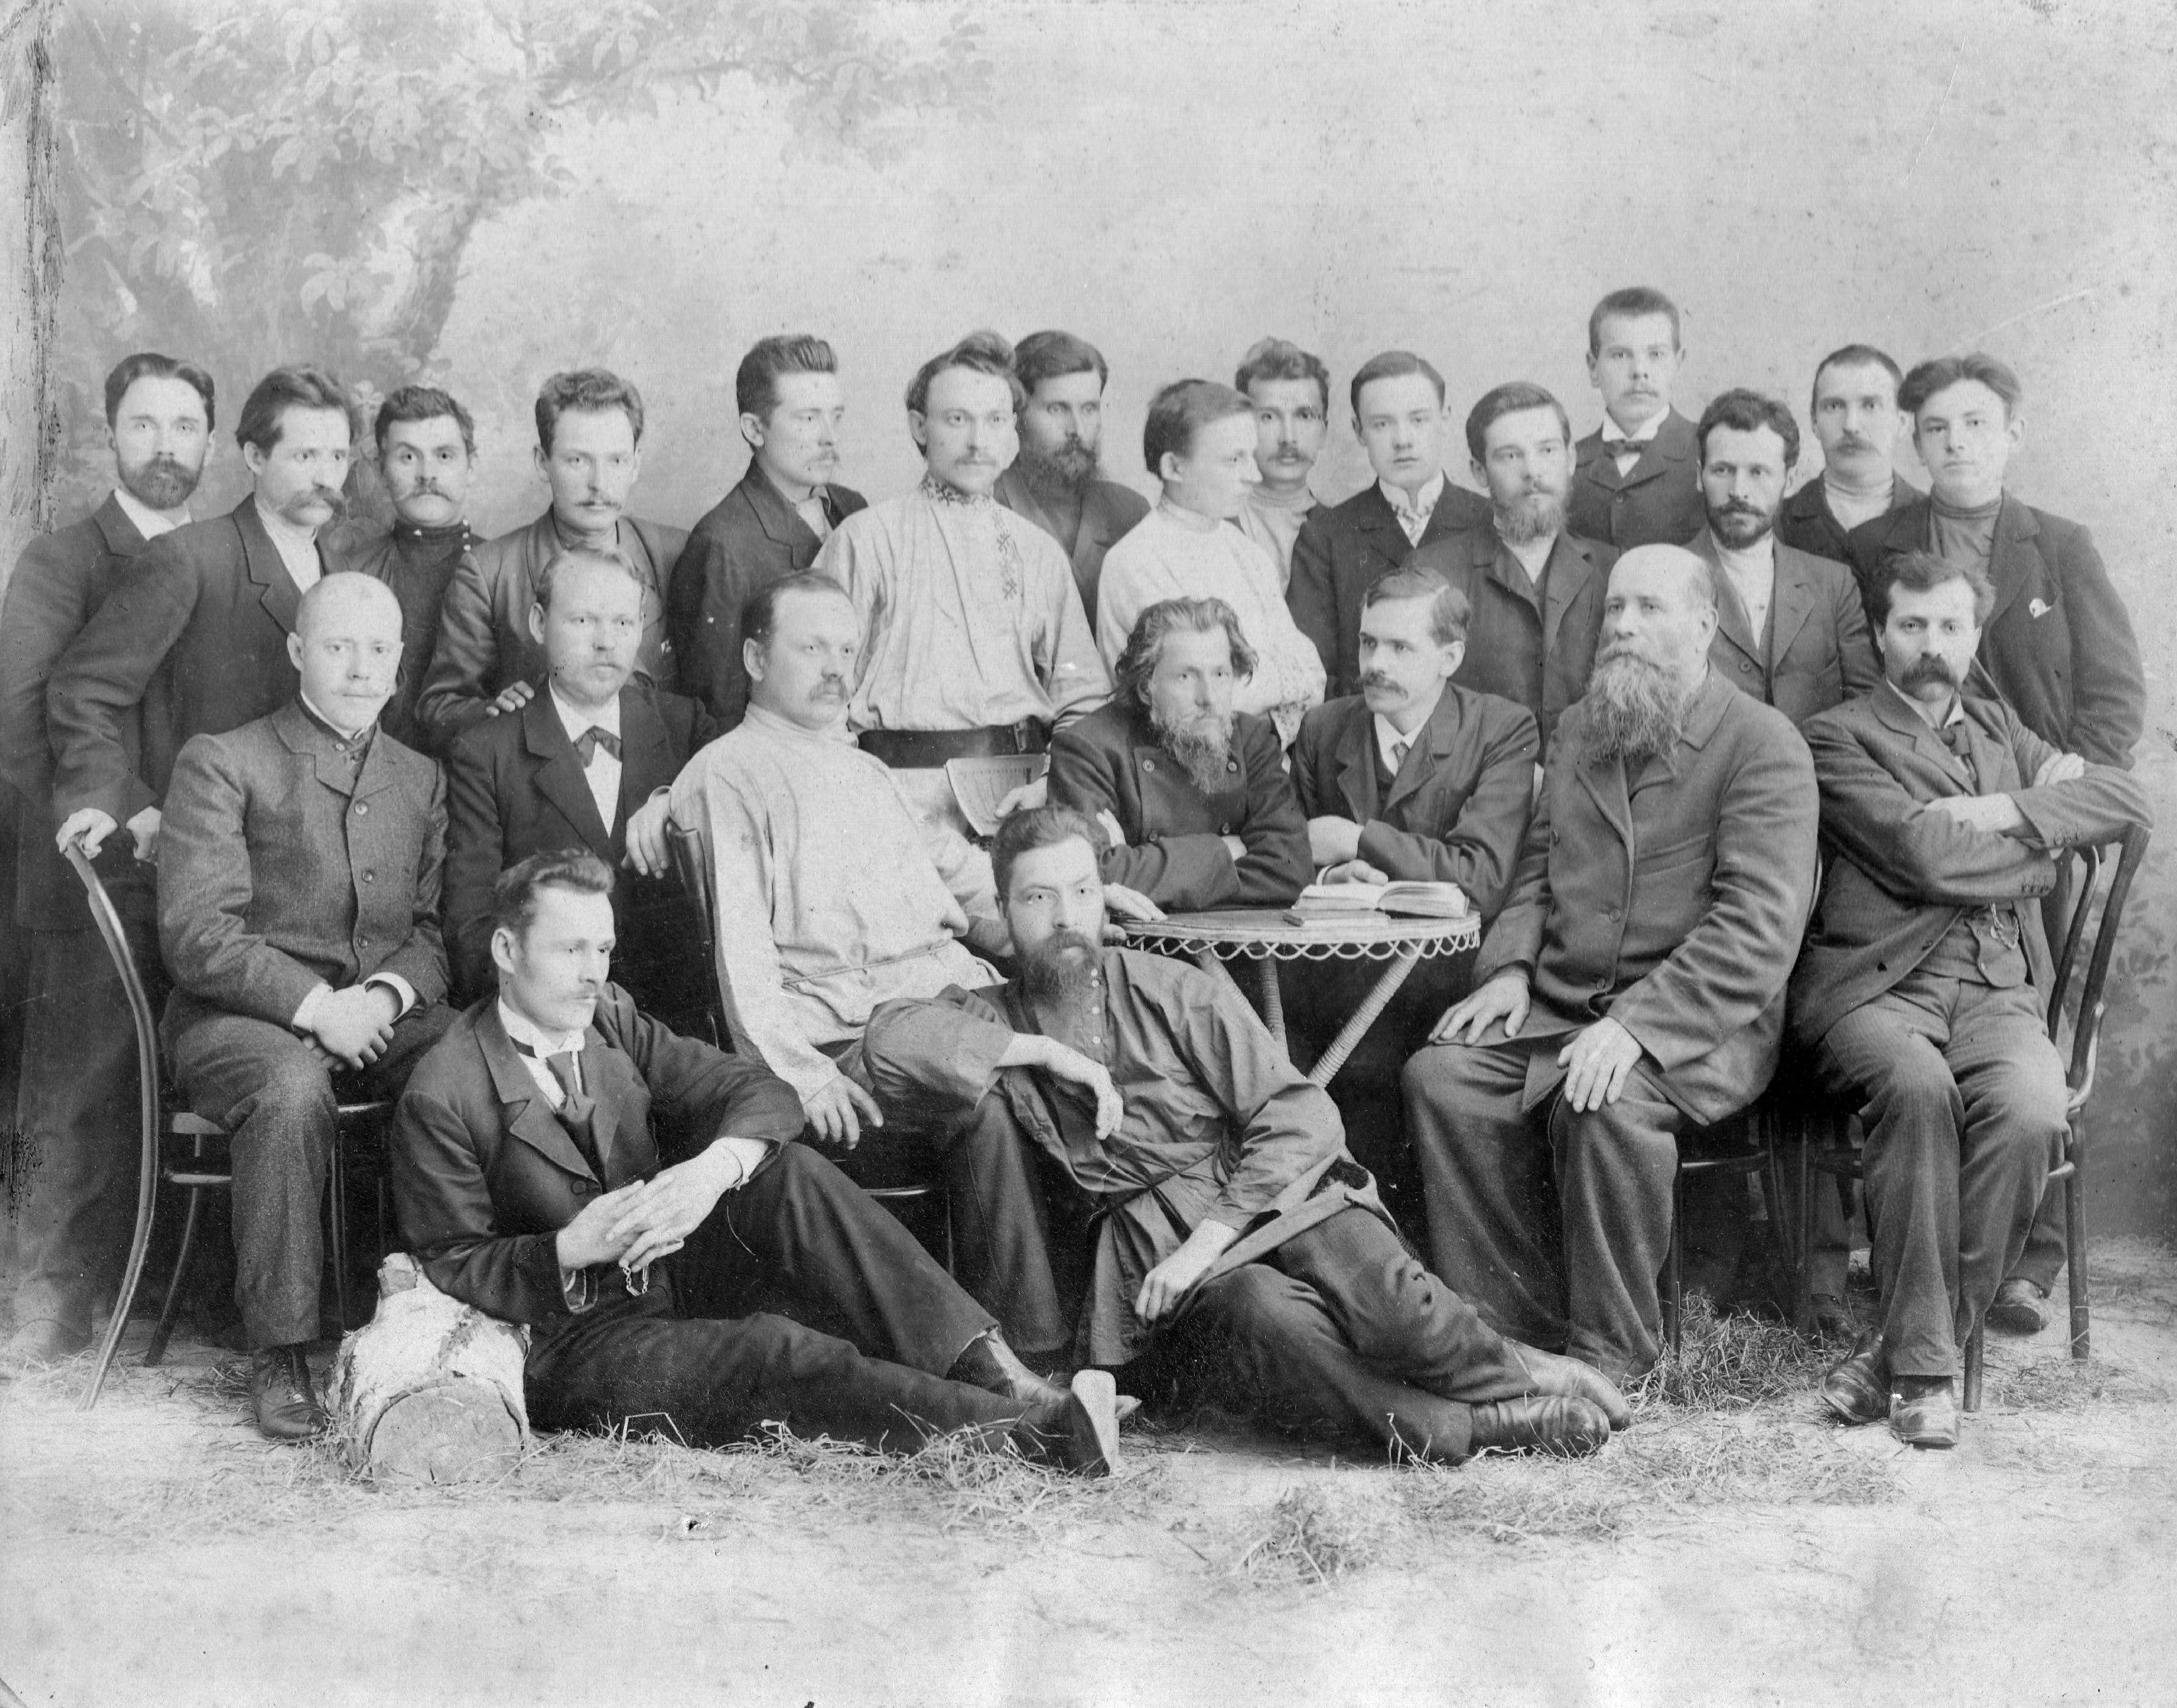
\includegraphics[width=0.9\textwidth]{pisateli.pdf}
  \caption*{Писатели и интеллигенция волоколамского уезда. Егор Кузьмичёв (4-й слева в последнем ряду), Федор Шкулев (2-й слева во втором ряду), Подъячев Семён (?) (3-ый справа во втором ряду), Спиридон Дрожжин (4-ий слева во втором ряду). Предположительно здесь есть Николай Михайлов, Сергей Ганьшин}
\end{figure}
